\documentclass{article}
\usepackage[utf8]{inputenc}
\usepackage[english]{babel}
\usepackage{fancyhdr}
\usepackage{graphicx}
 
\pagestyle{plain}
\fancyhf{}
\rhead{Version: 0.2}
\chead{Date: 2018-10-08, Doc. Number: PUSS18005}
\lhead{Resp.: SG}
\title{STLDD - Software Top Level Design Document}
\usepackage{enumitem}
\usepackage{lipsum}
\begin{document}

\author{SG}

\maketitle
\thispagestyle{fancy}
\tableofcontents
\newpage
\maketitle

\section*{Document history}
 \begin{tabular}{||c c c c||} 
 \hline
 Version & Date & Resp & Description \\ [0.5ex]
 \hline\hline
 0.1 & 2018-10-02 & SG & Draft version \\
 0.2 & 2018-10-08 & SG & Draft version 2 \\
 \hline
 

\end{tabular}

\section{Introduction}
This document describes the top-level design of the system. It is a system that helps commuters car pool between cities by matching drivers and commuters based on their departure locations and destinations, as well as the time of the commute. The users will be able to add the routes they will be driving and search for routes they would like to ride with somebody.

The system is developed by group 5 of the course ETSN05 2018.

\section{Reference documents}

\begin{enumerate}
    \item SRS - Software Requirements Specification, v. 1.0
    \item Documentation for the system. (Documentation.pdf)
    \item UML diagram for the system. (UML.png)
\end{enumerate}

\section{Overview}

This section contains a description of all the classes used for the database and backend in the application. Every subsection is a package in the project.

\subsection{Data}

This package contains classes that are a java representation of the data in the database.

\begin{description}
    \item[class User] This is a basic class to represent the data of a user from the Database.
    \item[class Location] This is a basic class to represent the data of a location from the Database.
    \item[class Ride] This is a basic class to represent the data of a ride from the Database.
    \item[class Role] This is a basic class to represent the data of a role from the Database.
    \item[class Session] This is a basic class to represent the data of a session from the Database.
    \item[class Credentials] This class handles the credentials of a user. Which is used to authorize the user to do certain actions. Example an user should only be able to have remove access to rides created by themselves.
    \item[class Date] This class hold the information of a date and time. Then formats in properly and returns the data throught getters.
    \item[class UserDataAccess] This DataAccess class extends the DataAccess superclass. It contains methods for all the actions that can be done to a user in the database.
    \item[class LocationDataAccess] This DataAccess class extends the DataAccess superclass. It contains methods for all the actions that can be done to a location in the database.
    \item[class RideDataAccess] This DataAccess class extends the DataAccess superclass. It contains methods for all the actions that can be done to a ride in the database.
\end{description}

\subsection{Database}

This package handles accessing and operations associated with the database.

\begin{description}
    \item[class CreateSchema] This class contains methods for creating the database schema. It is being used at start-up to make sure there exist one. If there isn't a schema, one is created.
    \item[class DataAccessException] This class is used to wrap in a SQLException and adds an ErrorType to the handled exception.
    \item[class DataAccess] This class is the superclass for all DataAccess classes. It provides access to the H2 database and contains helper methods for common JDBC use cases. Also contains a method for setting up the database schema.
    \item[class ErrorType] This is used to communicate to client about usage errors without exposing underlying implementation details.
    \item[class Mapper] This is a helper class which is used to make working with JDBC's checked exception easier.
    \item[class MapMapper] This class is used for debugging SQL queries without having to write a fixed Mapper.
\end{description}

\subsection{Rest}

This package is a link between the front-end and the back-end. Enabling the user to do calls to the database from the webpage.

\begin{description}
    \item[class UserResources] This class is a link between the user using the Front-End trying to communicate with the Database. It's a rest API and this class specifically handles actions related to a user.
    \item[class LocationResources] This class is a link between the user using the Front-End trying to communicate with the Database. It's a rest API and this class specifically handles actions related to a location.
    \item[class RideResources] This class is a link between the user using the Front-End trying to communicate with the Database. It's a rest API and this class specifically handles actions related to a ride.
\end{description}

\subsection{Provider}

The classes in this package are support classes. Used to convert object to Json and adding session to http requests.

\begin{description}
    \item[class AuthenticationFilter] Adds the Session to the current HTTP request to the REST API. This is done by extracting the token in the users cookie and checking the database for the cookie.
    \item[class JsonProvider] This class is a converter of all the objects in the REST API between Java Object and Json Object. It uses Gson.
    \item[class JsonExceptionMapper] This converts all Exceptions to HTTP responses for the REST API. It has special handling for WebApplicationException and DataAccessException.
\end{description}

\subsection{Ranker}

This package contains only one class. It is used to rank different rides, to present them in a better manner for the user.

\begin{description}
    \item[class Ranker] This class ranks every ride in a list of rides and return a sorted list based on those rankings. It can rank on several different criteria depending on where it's used.
\end{description}

\subsection{Front-End}

The front-end will be done in JavaScript, HTML and CSS. And will build upon the base system provided by LTH. Each tab will be described in it's own file. 

\section{Class diagram}
The system's architecture is described by the UML diagram shown in Figure \ref{fig:uml}.
There is a higher resolution version of the diagram located in the same folder as this document called UML.png.

All classes and public methods are described in the document Documentation.pdf, also located in the same folder as this document.

\section{Database}
    There is one database with four tables;
    
    Users, Locations, Rides and PassengerRides.
\subsection{ER-Diagram}
The database is described by the ER-diagram in Figure \ref{fig:er}.
\begin{figure}[h]
  \centering
  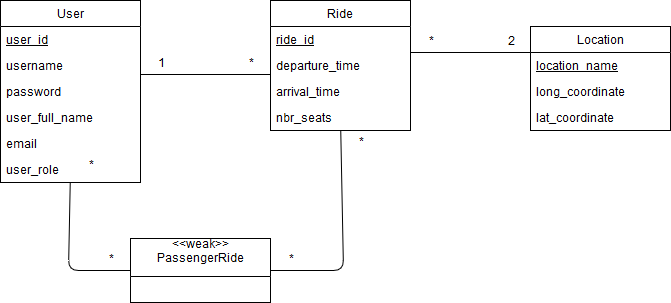
\includegraphics[scale=0.52]{ERDiagram.png}
  \caption{ER-diagram of the database}
  \label{fig:er}
\end{figure}

\subsection{ER-Relations}
%Lite osäker på namnen men detta är ett utkast.
The following ER-relations describe the database used by the system. Primary keys are \underline{underlined} and foreign keys are written in \textit{italics}.
\\ \\
Users (\underline{user\_id}, username, password, user\_full\_name, user\_email, user\_role)
\\
Locations (\underline{location\_name}, long\_coordinate, lat\_coordinate)
\\
Rides (\umderline{ride\_id}, departure\_time, arrival\_time, nbr\_seats, \textit{driver\_id, departure\_location, destination})
\\
RidePassengers (\underline{\textit{ride\_id, passenger\_id}})
\\ \\
The table "users" contains information about all users of the system. "user\_roles" indicates whether the user is an administrator or a regular user of the system.

"locations" holds information about the locations that rides can go between.

"rides" contains the information about each ride, excluding its passengers. These are stored in the table "ridePassengers" for all rides.

\subsection{SQL-code}
The following code should be used to create the tables.

\begin{verbatim}
    CREATE TABLE users (
        user_id INT AUTO_INCREMENT NOT NULL,
        username VARCHAR NOT NULL UNIQUE,
        password VARCHAR NOT NULL,
        user_full_name VARCHAR NOT NULL,
        email VARCHAR NOT NULL,
        user_role VARCHAR NOT NULL,
        PRIMARY KEY (user_id));
    
    CREATE TABLE locations (
        location_name VARCHAR NOT NULL,
        long_coordinate INT NOT NULL,
        lat_coordinate INT NOT NULL,
        PRIMARY KEY (location_name));
        
    CREATE TABLE rides (
        ride_id INT AUTO_INCREMENT NOT NULL,
        departure_time DATE NOT NULL,
        arrival_time DATE NOT NULL,
        nbr_seats INT NOT NULL,
        driver_id INT NOT NULL,
        departure_location VARCHAR NOT NULL,
        destination VARCHAR NOT NULL,
        PRIMARY KEY (ride_id),
        FOREIGN KEY (driver_id) REFERENCES users (user_id),
        FOREIGN KEY (departure_location) REFERENCES locations (location_name)
        FOREIGN KEY (destination) REFERENCES locations (location_name));
    
    CREATE TABLE ridePassengers (
        ride_id NOT NULL,
        passenger_id NOT NULL,
        PRIMARY KEY (ride_id, passenger_id),
        FOREIGN KEY (ride_id) REFERENCES rides (ride_id),
        FOREIGN KEY (passenger_id) REFERENCES users (user_id));
        
\end{verbatim}

\section{Sequence diagrams}

\begin{figure}[h]
  \centering
  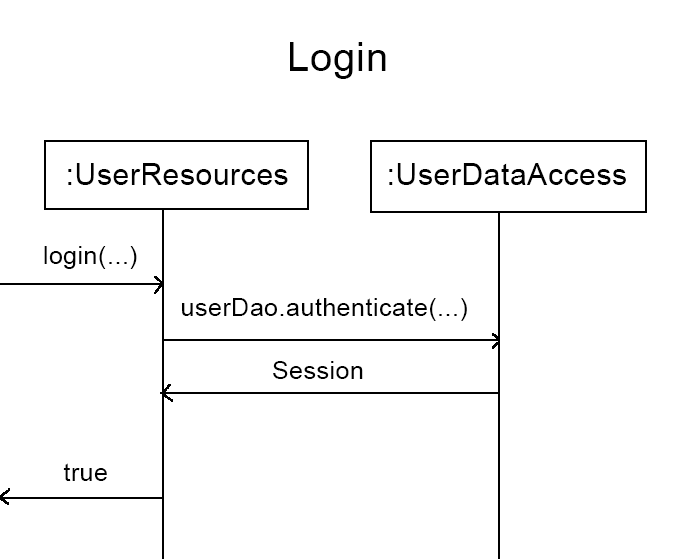
\includegraphics[scale=0.3]{seqdiagram1.png}
  \caption{Sequence diagram of login procedure.}
  \label{fig:seq1}
\end{figure}

\begin{figure}[h]
  \centering
  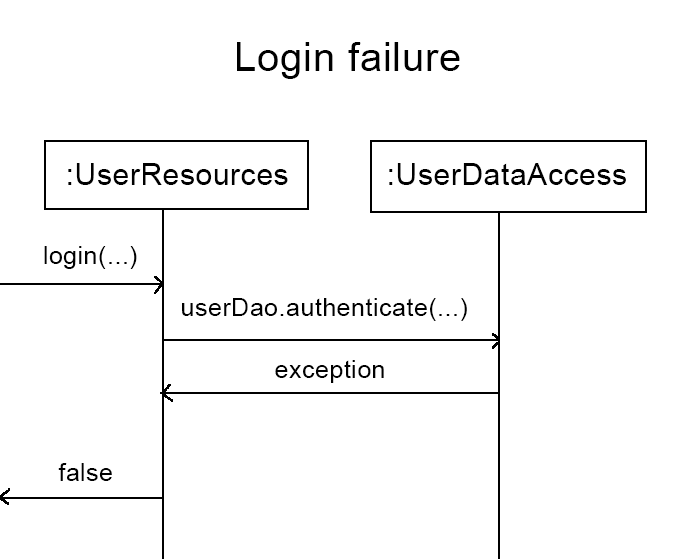
\includegraphics[scale=0.3]{seqdiagram2.png}
  \caption{Sequence diagram of failure of login procedure.}
  \label{fig:seq2}
\end{figure}

\begin{figure}[h]
  \centering
  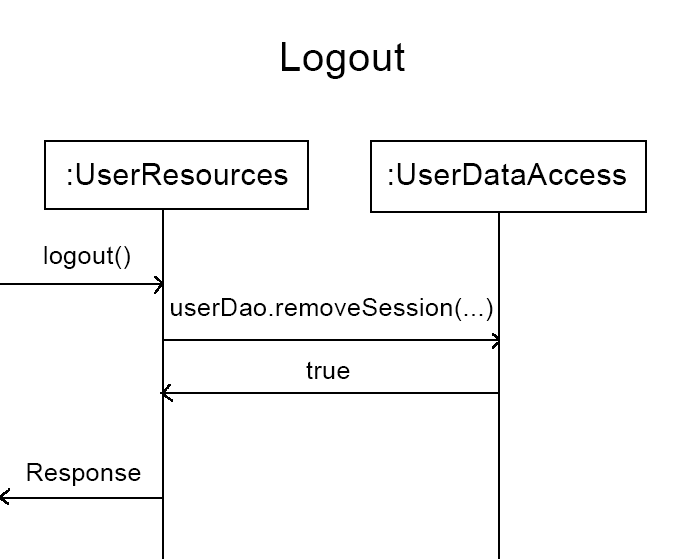
\includegraphics[scale=0.3]{seqdiagram3.png}
  \caption{Sequence diagram of logout procedure.}
  \label{fig:seq3}
\end{figure}

\begin{figure}[h]
  \centering
  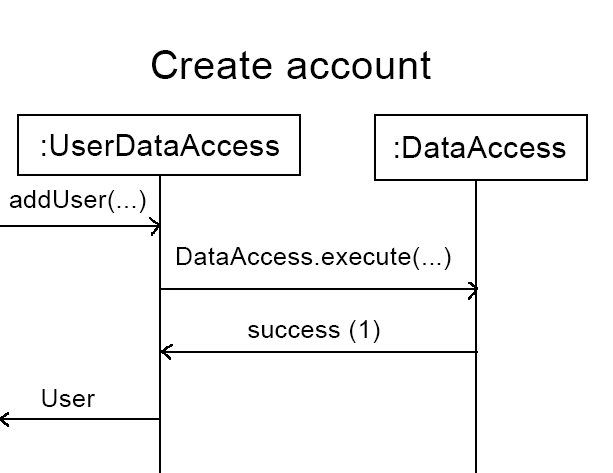
\includegraphics[scale=0.2]{seqdiagram4.png}
  \caption{Sequence diagram of the procedure of creating an account.}
  \label{fig:seq4}
\end{figure}

\begin{figure}[h]
  \centering
  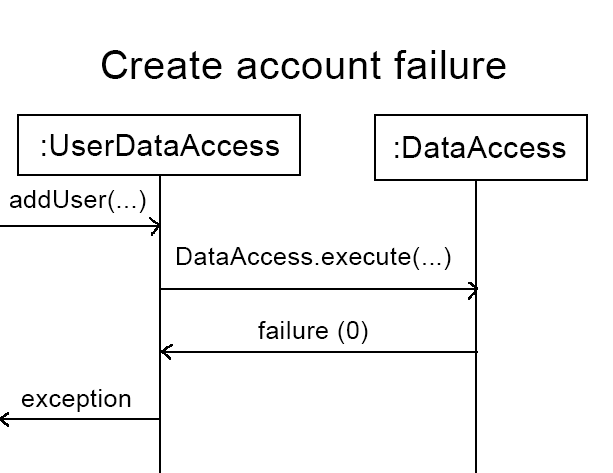
\includegraphics[scale=0.3]{seqdiagram5.png}
  \caption{Sequence diagram of failing to create an account.}
  \label{fig:seq5}
\end{figure}

\begin{figure}[h]
  \centering
  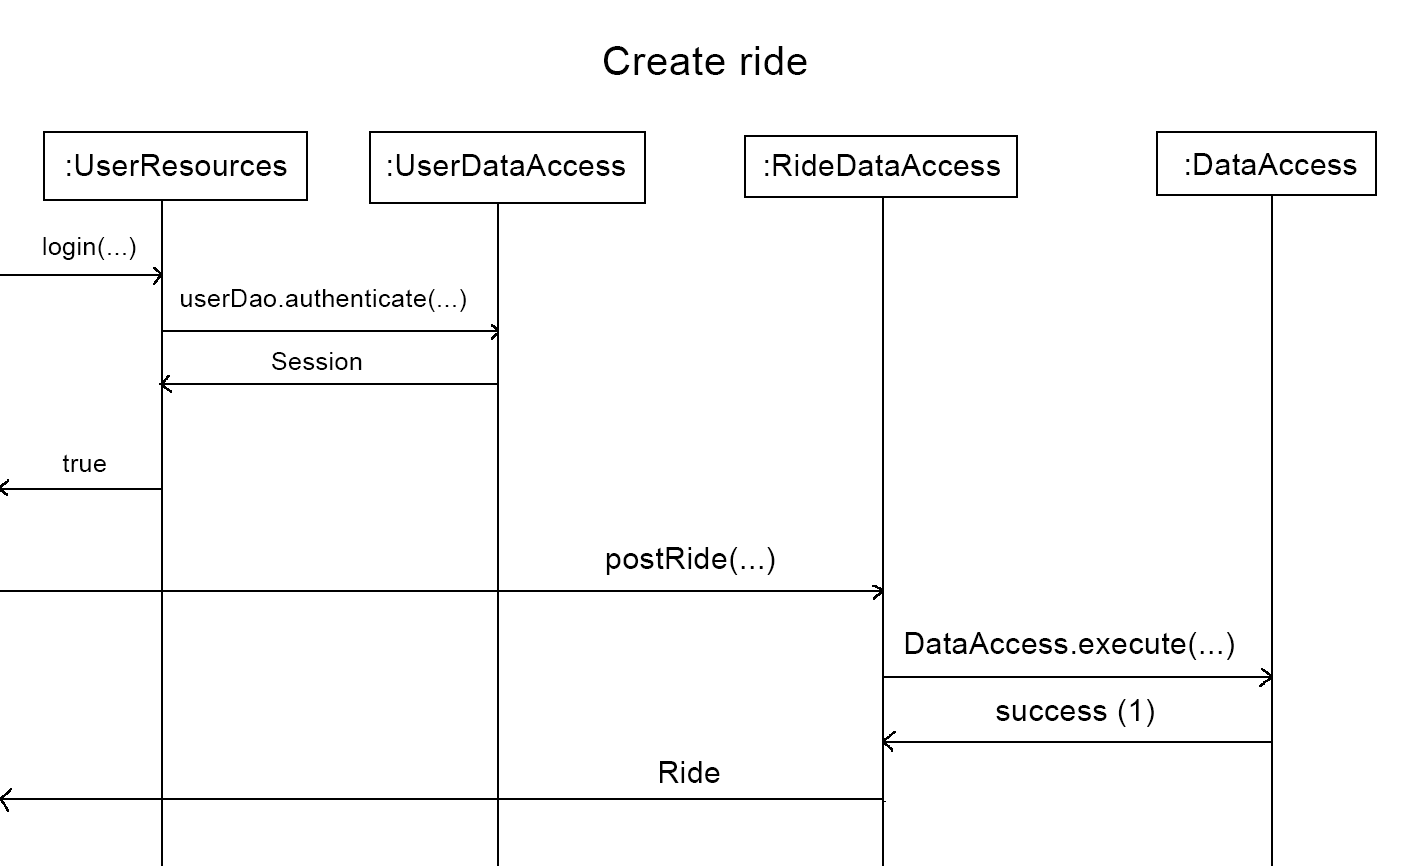
\includegraphics[scale=0.3]{seqdiagram6.png}
  \caption{Sequence diagram of creating a ride.}
  \label{fig:seq6}
\end{figure}

\begin{figure}[h]
  \centering
  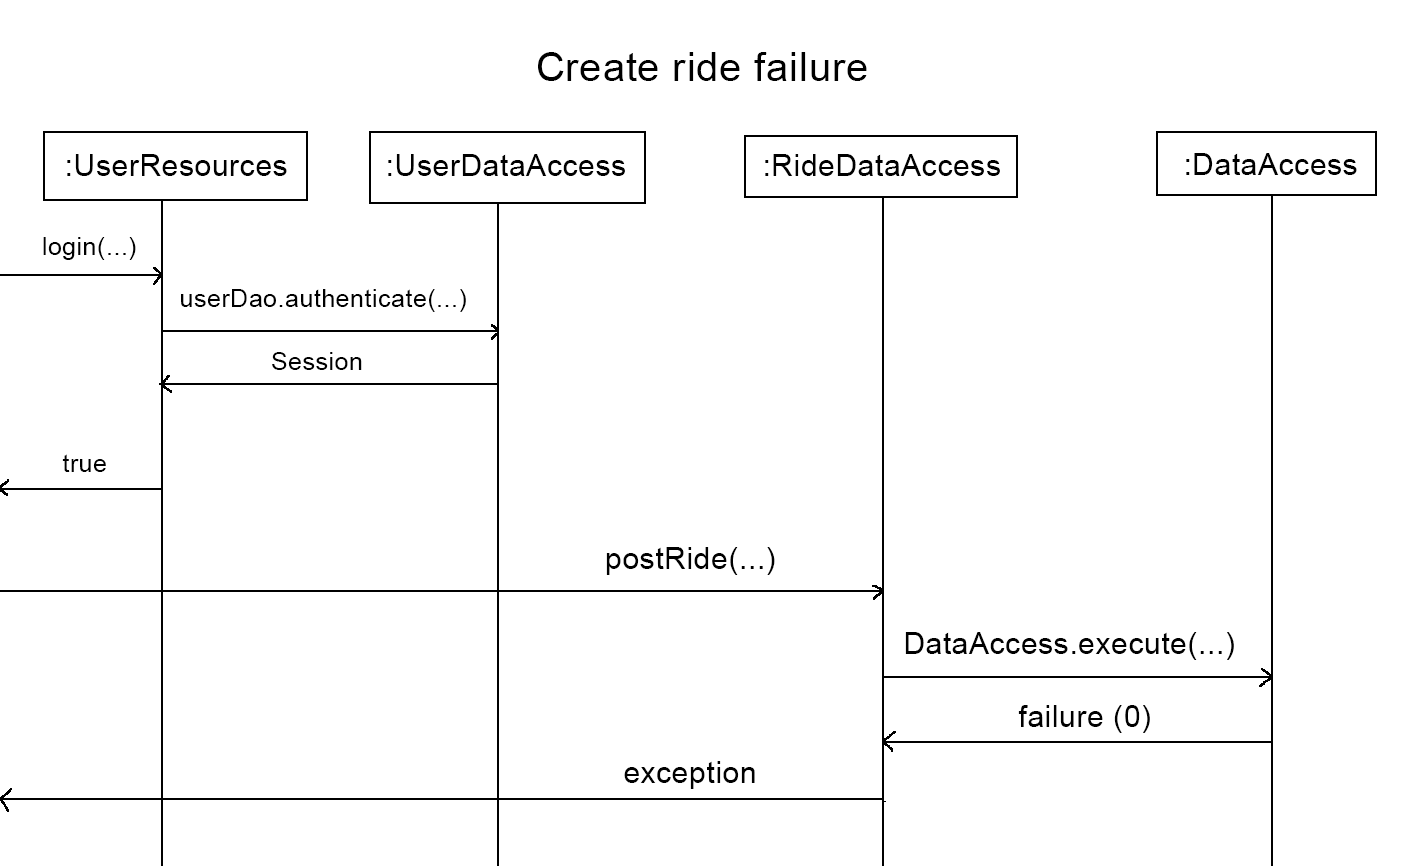
\includegraphics[scale=0.25]{seqdiagram7.png}
  \caption{Sequence diagram of failing to create a ride.}
  \label{fig:seq7}
\end{figure}

\begin{figure}[h]
  \centering
  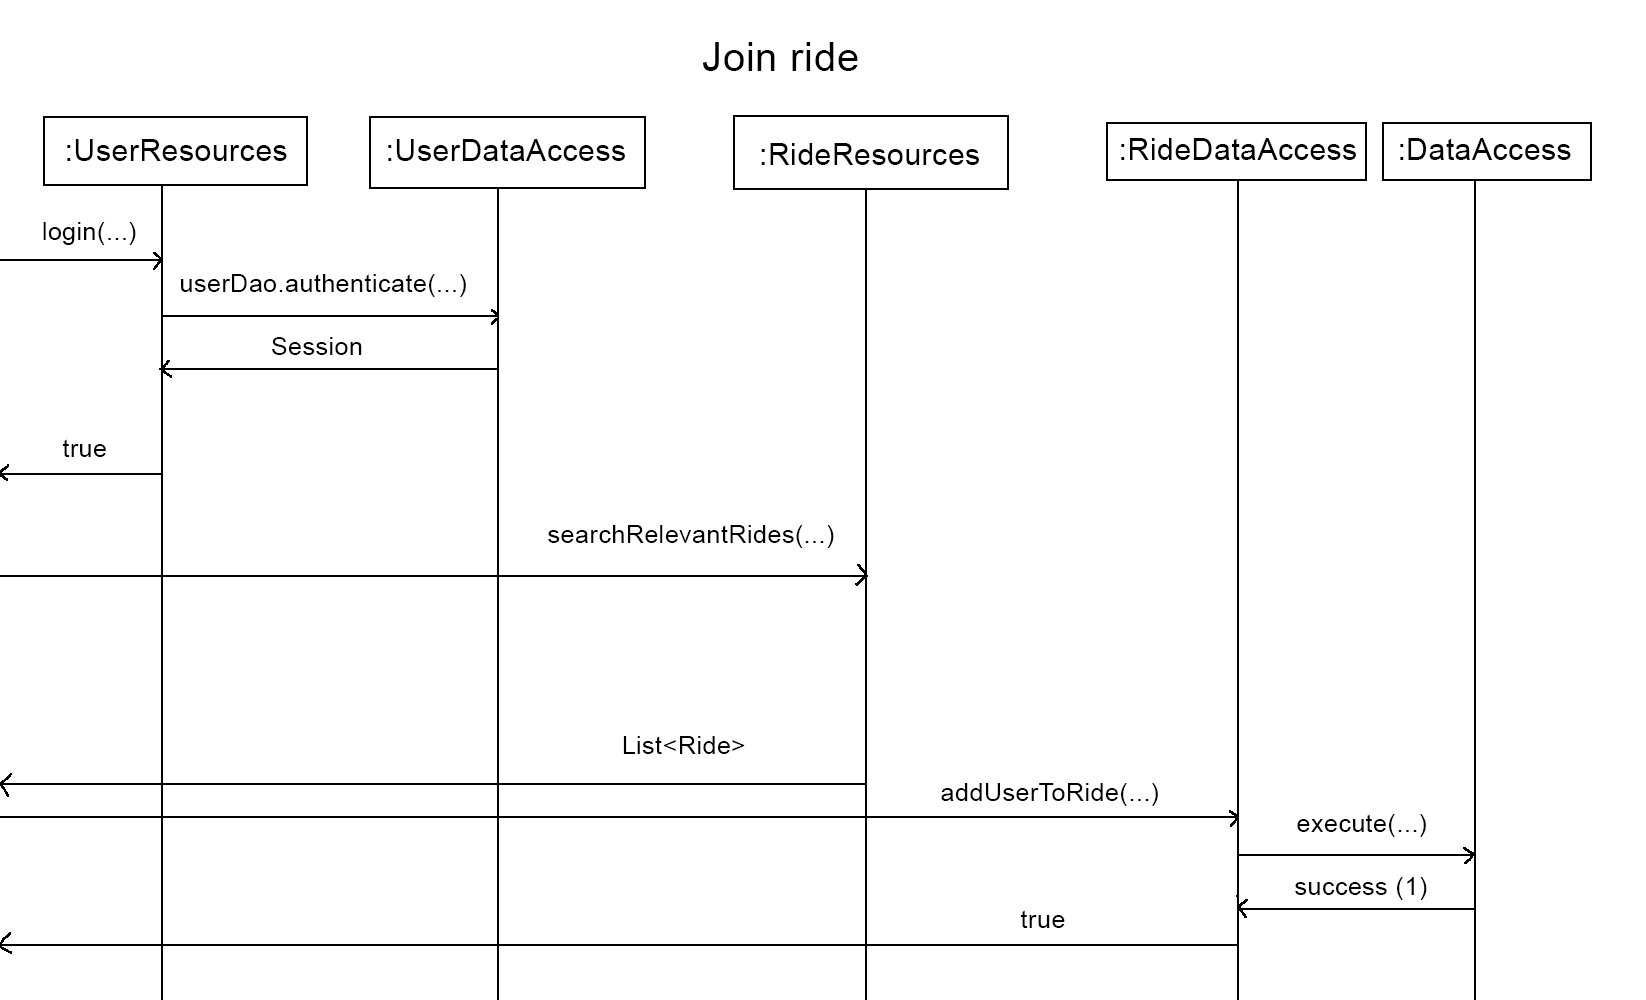
\includegraphics[scale=0.25]{seqdiagram8.png}
  \caption{Sequence diagram of joining a ride.}
  \label{fig:seq8}
\end{figure}

\begin{figure}[h]
  \centering
  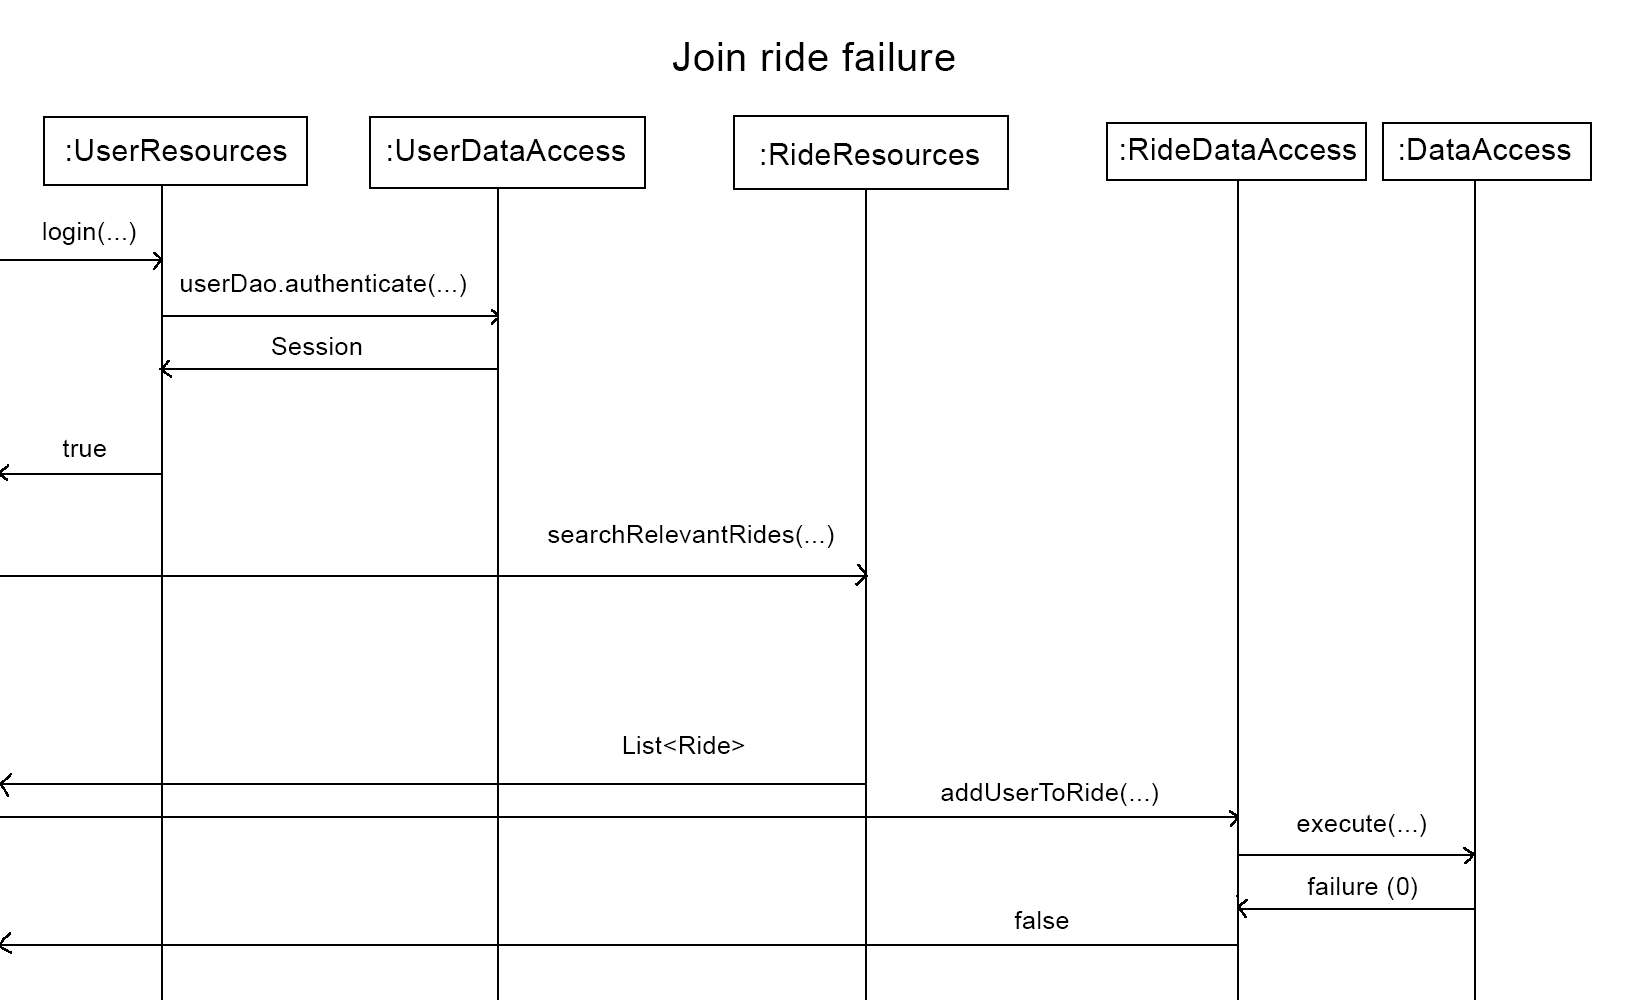
\includegraphics[scale=0.25]{seqdiagram9.png}
  \caption{Sequence diagram of failing to join a ride.}
  \label{fig:seq9}
\end{figure}

\newpage
\begin{figure}[h]
  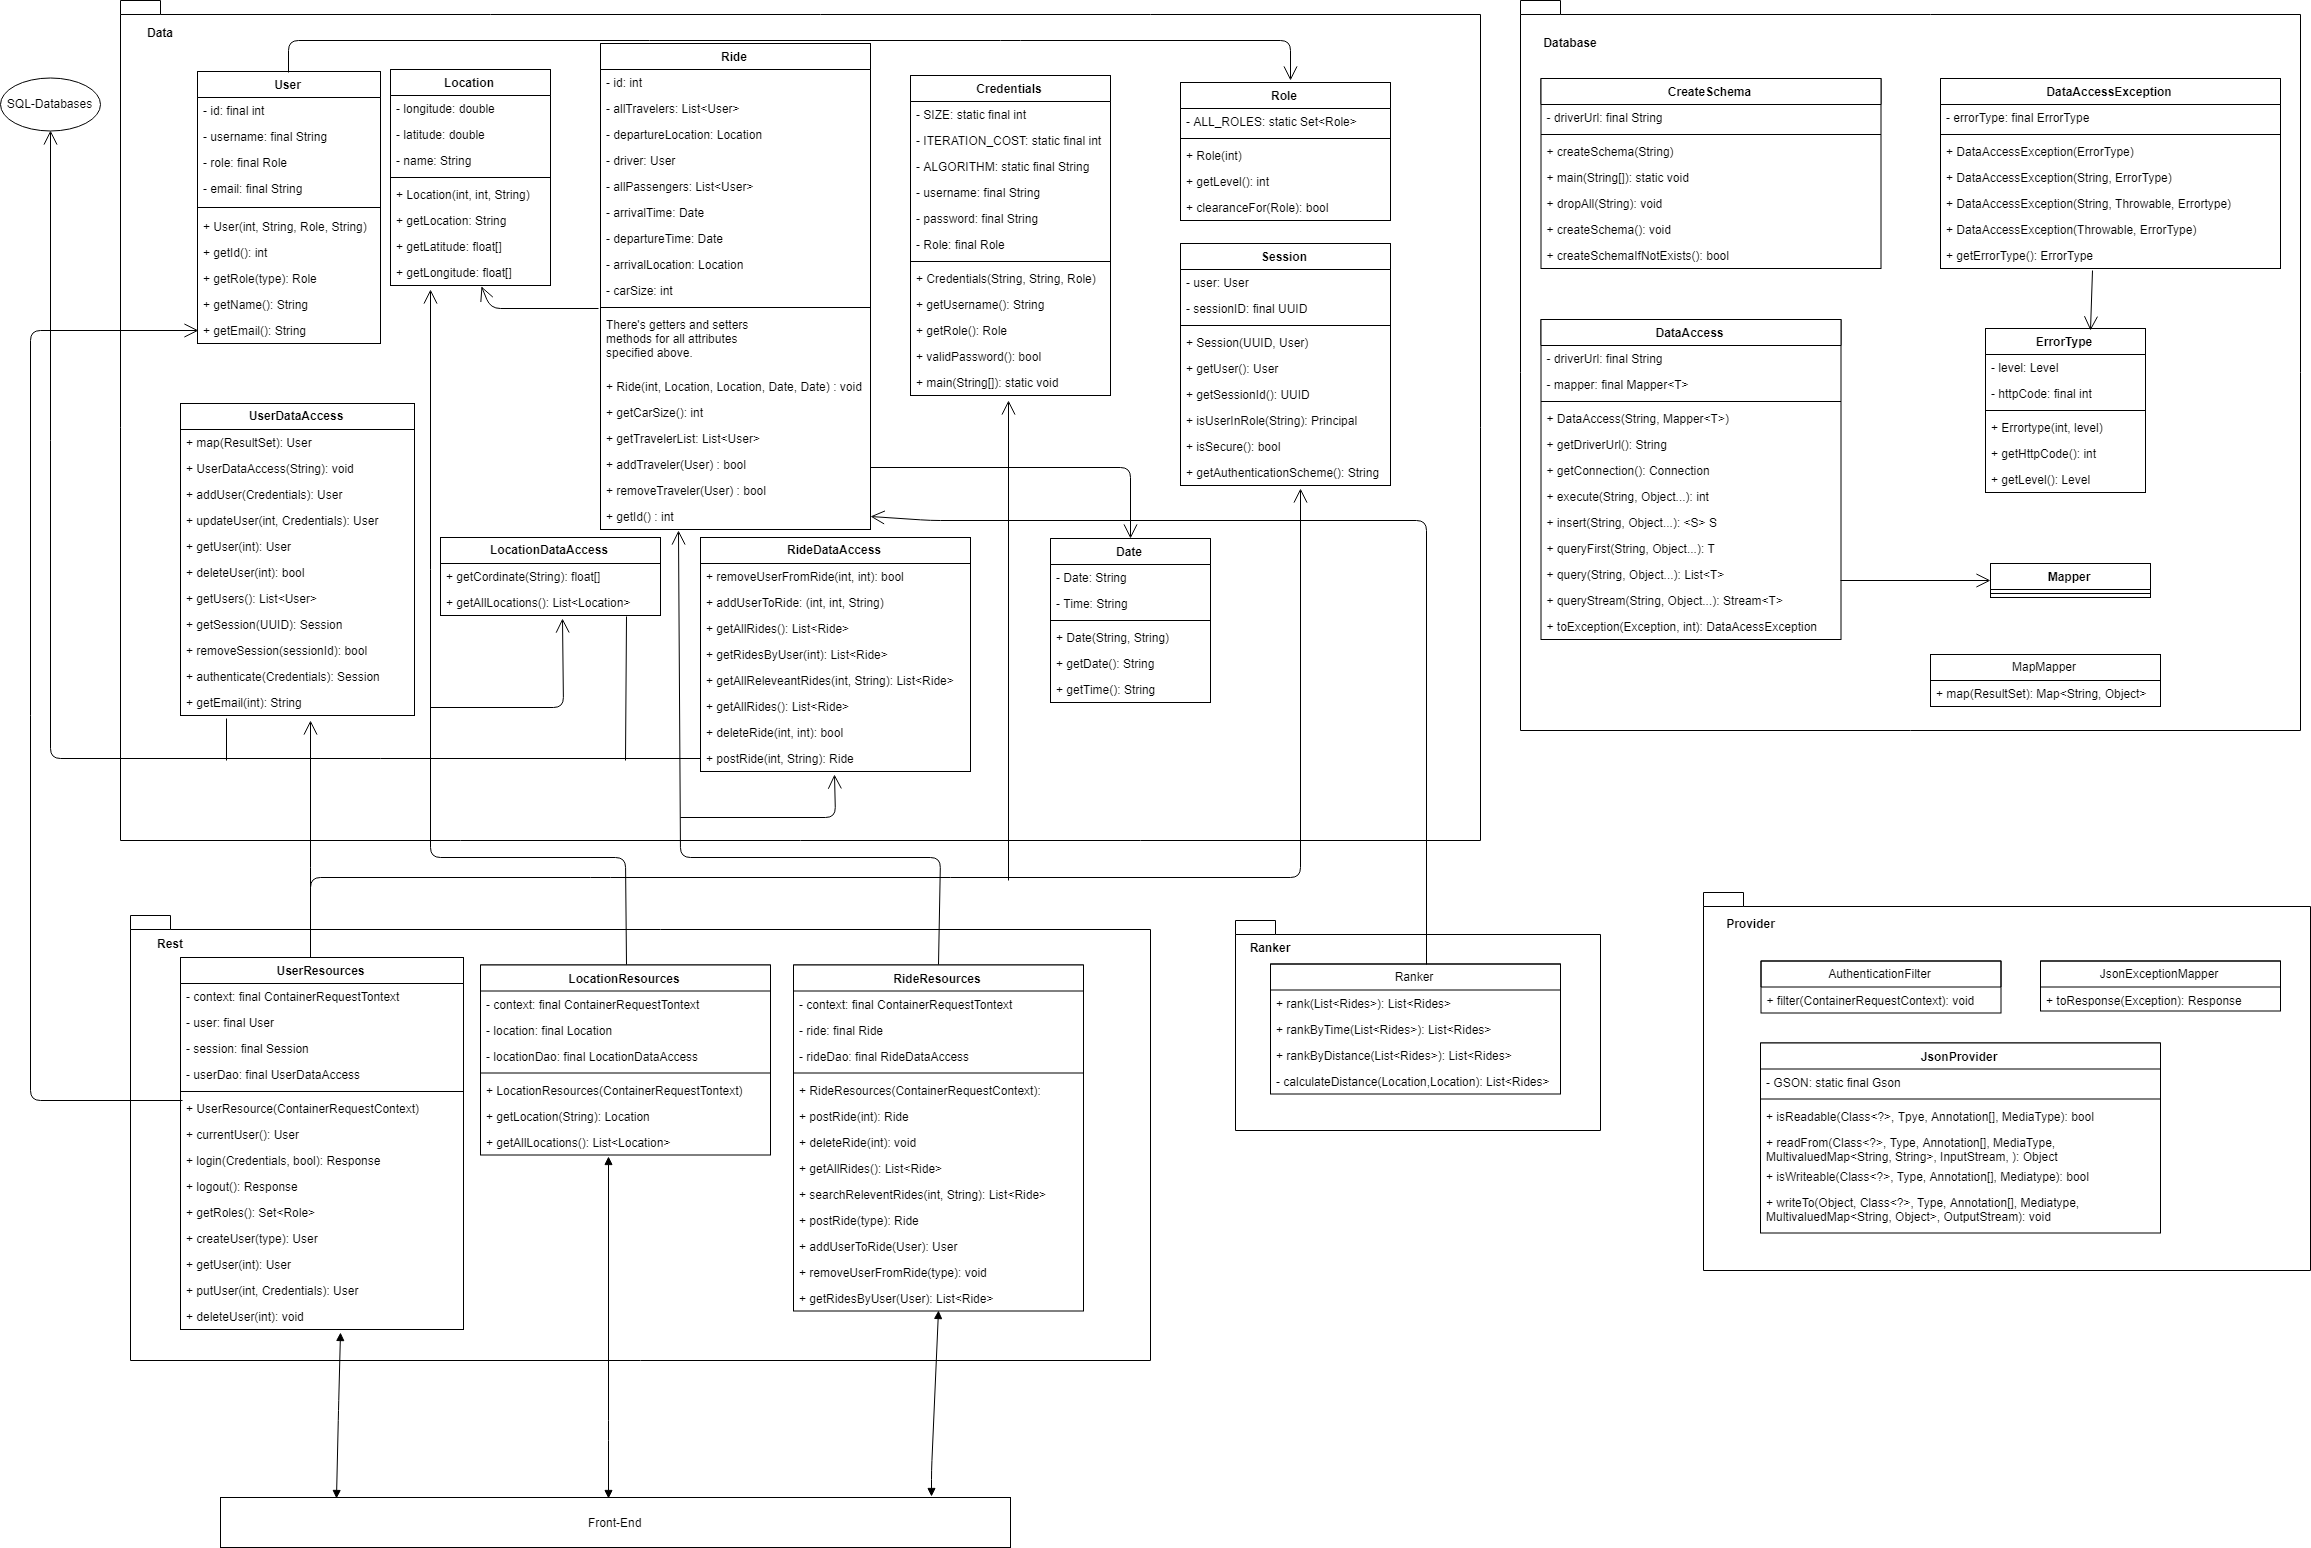
\includegraphics[scale=0.27, angle=90]{UML.png}
  \caption{UML describing the system(source: }
  \label{fig:uml}
\end{figure}

\end{document}
